\documentclass{article}
%\usepackage[T1]{fontenc}
%\usepackage[utf8]{inputenc}
\usepackage{enumerate}
\usepackage{multirow}
\usepackage[bottom,flushmargin,hang,multiple]{footmisc}
\usepackage{etoolbox}
\makeatletter
\patchcmd\maketitle{\hb@xt@1.8em}{\hbox}{}{}
\makeatother
\patchcmd{\maketitle}{\@fnsymbol}{\@arabic}{}{}
\usepackage{amsmath}
\usepackage{graphicx}
\usepackage{caption}
\usepackage{subcaption}
\usepackage[margin=1.25in]{geometry}
\usepackage{float}
\usepackage{comment}
\usepackage{pgf}
\linespread{1.5}

\usepackage{tikz}
\usepackage{subcaption}

\usepackage[T1]{fontenc}
\usepackage[sfdefault,scaled=1.05,light]{FiraSans}
\usepackage{newtxsf}

%\usepackage{url}
%\usepackage[square,sort,comma,numbers]{natbib}

\parindent=0pt
\usepackage{etoolbox}
\AtBeginEnvironment{quote}{\small}

\newcommand{\Vx}{\textbf{Var}_x}
\newcommand{\Ex}{\textbf{E}_x}
\newcommand{\Vz}{\textbf{Var}_z}
\newcommand{\Ez}{\textbf{E}_z}
\newcommand{\x}{\mathbf{x}}
\newcommand{\z}{\mathbf{z}}

% \renewcommand{\familydefault}{lmodern}
\begin{document}


\title{Assessing latent variables models by studying the moment estimator gap}

%\subtitle{Poste de professeure, professeur en statstique et science des données}

%\titlerunning{Short form of title}        % if too long for running head

\author{C\'edric Beaulac}


\date{\today}
% The correct dates will be entered by the editor

\maketitle


\section{Introduction} \label{intr}

When fitting supervised models, statisticians and computer scientist alike have come up with tons of metrics in order to evaluate the quality of their predictions and judge their adequacy, from simple mean-squared error to more general loss functions. However, in the context of unsupervised learning there is no direct measure of success and it can be difficult to assess the validity of the fitted model \cite{Hastie09}.

\bigskip

In this article we propose a new way to assess the quality of the fit a large family of unsupervised models. More precisely, we offer a diagnostic technique for parametric latent variable models such as Variational AutoEncoders (VAEs) \cite{Kingma13,Kingma17} and Gaussian Mixture Models (GMMs). Our proposed metrics evaluates the quality of the \textit{fitted model}; we compare the learned parameters of the unsupervised model with the observed data distribution the model is trying to capture. We do so by building two distinct moment estimators. 

\bigskip

The technique we propose is fast to compute, works for a wide range of models and is built upon a rigorous mathematical formulation. It provides a new way to compare multiple models and behave accordingly to previously used heuristic techniques.

\bigskip

In the next section we establish the family of latent variable model suited for this metric. After we discuss related work in section \ref{rewo}, we discuss the moments estimators used in section \ref{moes}.  In section \ref{mega}, we present our metric. We show how this metric perform with simulations in section \ref{expe}. Finally, section \ref{fuwo} propose a wide range of future application of the ideas presented in this article such as the possibility of training models using the proposed metric. 

\section{Latent variable generative models}\label{lvgm}

The diagnostic tool we propose is useful to assess the quality of the fit for a family of unsupervised latent variable models. In this section we define this family, the Latent variable generative models (LVGMs).

\bigskip

Assuming we have a data set $S= \{\mathbf{x}_1,...,\mathbf{x}_N\}$ consisting of $N$ observations of a $D$-dimensional variable $\mathbf{x}$. We assume $\x$ lives in the data-space $\mathcal{X}$ which is $D$-dimensional. We want to estimate the distribution of the random variable $\mathbf{x}$ but it is \textit{too complicated} to be captured by a simple distribution. Latent variable models suppose there exist a unobserved latent variable, say $\mathbf{z}$, that has a direct influence on the distribution of $\mathbf{x}$:
\begin{align}
p(\x) = \int_{z} p(\x|z)p(\z) dz
\label{LVM}
\end{align}
where we assume $\z$ is in lives in a latent-space $\mathcal{Z}$ which is $M$-dimensional. The model proposed by equation \ref{LVM} is quite general but allows relatively complex marginal distributions over observed variables $\mathbf{x}$ to be expressed in terms of more tractable conditional distributions $p(\x|z)$ \cite{Bishop07}. Similarly, it leads to a tractable joint distribution as well:
\begin{align}
p(\x,\z) = p(\z)p(\x|z)
\label{jointLVM}
\end{align}

and is quite often represented using a simple graph:
\begin{figure}[h!]
  \centering
  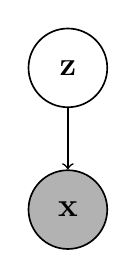
\begin{tikzpicture}[->, semithick,scale = 0.9]
  \tikzstyle{latent}=[fill=white,draw=black,text=black,style=circle,minimum size=1.0cm]
  \tikzstyle{observed}=[fill=black!30,draw=black,text=black,style=circle,minimum size=1.0cm]

  \node[latent] 		(A)	at (0,2)		{\large $\mathbf{z}$};

  \node[observed]         (C)	at (0,0)		{\large $\mathbf{x}$};

        
  \path (A) edge            node {} (C);


\end{tikzpicture}
  \caption{Graphical representation of latent variables models with joint distribution $p(\mathbf{x},\mathbf{z}) = p(\mathbf{z})p(\mathbf{x}|z)$.}
  \label{genny}
\end{figure}%
These models are \textit{generative models} because learning $p(\x,\z)= p(\z)p(\x|z)$ allows us to generated new samples of $\x$ using ancestral sampling. What makes this model probabilistic is that the mapping from $\z$
 to $\x$ is not a deterministic function $f: \mathcal{Z} \rightarrow \mathcal{X}$ but instead a \textit{probabilistic mapping} from $\mathcal{Z}$ to the parameter space $\Theta$, where $\Theta$ is the parameter space of $p_\theta(\x|z)$; $\theta \in \Theta$. We will call $p_\theta(\x|z)$ the emission distribution or observation distribution interchangeably.
 
\bigskip

When training or fitting such models we are training the function $f:\mathcal{Z} \rightarrow \Theta$ in ways to maximize the likelihood of the data set $S$ under the model of equation \ref{LVM}. This mapping $f$ explains the effect of $\z$ on $\x$ ans is at the centre of latent variable models. Learning this function $f$ is the main challenge of optimizing latent variable model and the Expectation-Maximization algorithm (EM) or variational inference are common strategies to fit learn such function. In most cases, $p(\z)$ is assumed to be known and fixed but in some cases the parameters of $p(\z)$ are estimated as well.

\bigskip

Usually $p_\theta(\x|z)$ is a simple parametric distribution and the latent variable is in charge of increasing the complexity of $p_\theta(\x)$. Additionally, the function $f$ can take many forms, from simple linear combination to neural network functions. We will use $f(\z)$ interchangeably with $f$ but also sometimes the \textit{distribution parameters} it outputs directly. For the majority of emission distribution we consider, there exist a simple mapping from the parameters of the distribution to its expectation and its variance.

\bigskip

For instance, assuming the emission distribution is Poisson: $p_\theta(\x|z) = \text{Poisson}(\lambda)$ then $f: \mathcal{Z} \rightarrow \mathbb{R}^+$ and we might use $f(\z)$ and $\lambda(\z)$ interchangeably. Additionally, $\Ex[\x|\z] = \lambda(\z)$ and $ \Vx[\x|\z] = \lambda(\z)$. 


\subsection{Probabilistic Principal Component Analysis}

The Probabilistic Principal Component Analysis (pPCA) \cite{tipping99,Bishop07} is a member of the LVGM family we just described where $p(\z)$ is assumed to be a normal distribution $N(0,I)$. We also assume the emission distribution to be Normal: $p(\x|\z) = N(W\z+\mu,\sigma^2I)$. In this formulation, we see that $f: \mathbb{R}_M \rightarrow \mathbb{R}_D$ is a linear function that maps the latent variable $\z$ to $\Ex[\x|\z]$. Outside of estimating $W$ and $\mu$ as part of $f$ the model also estimate $\sigma^2$ though it is not a function of $z$. However it is function of $D$ and $M$, the dimension of $\mathcal{X}$ and $\mathcal{Z}$. 

\bigskip

The parameters of pPCA can be fit analytically as the solution of a direct maximization of the likelihood or with the EM algorithm.   

\subsection{Variational AutoEncoders}

\subsection{Gaussian Mixture Models}

For a GMM with $K$-components we define $\z$ as a k-class categorical variable, $\z \in \{1,...,K\} = \mathcal{Z}$, $p(\z)$ is a categorical distribution where we define $\pi_j$ as $p(\z = j)$ with $\sum_{j=1}^K \pi_j =1$. Finally, setting $p(\x|z=j) = N(\mu_j,\sigma_j)$ leads to a GMM:
\begin{align}
p(\x) = \sum_{j=1}^K \pi_j p(\x|z=j) 
\label{LVM}
\end{align}
In this situation, $f$ map the latent variable to a pair of \textit{distribution parameters}, $\mu$ and $\sigma$, $f: \{1,...,K\} \rightarrow \mathbb{R}\times\mathbb{R}^+$. In this particular cases  $\Ex[\x|\z] = f_1(\z)$ where $f_1$ is the \textit{first} output of $f(\z)$ and $\Vx[\x|\z] = f_2(\z)$.

\bigskip

The GMM is a special case of LVGM where we also estimate the parameters $\{\pi_j : j \in 1,...K\}$ of $p_(\z)$. A GMM is usually train using the EM algorithm. 

\section{Related Works} \label{rewo}

We propose a metric to evaluate to goodness-of-fit of the family of latent variable define in section \ref{lvgm} and based on the literature there is no good metric for such thing at the moment. 

\bigskip

In the literature the likelihood of the data $S$ under the fitted model is used CITE, however,it has been shown CITE that sometimes a model can reach very high-likelihood even for terrible fit. For instance, Bishop et al. \cite{Bishop07} demonstrate that for   

\section{Moment estimators} \label{moes}

\subsection{Second moment}

We propose to build two different estimators of the same value. One uses observed data and the other uses the proposed generative model. What makes our model estimator different is that we do not generate points from the generative model but instead we rely on a simple probability identity to build the \textit{model} estimator. The estimator 

\bigskip

To do, let us introduce the well-know Law of Total Variance :


\begin{align}
\Vx(\x) = \Ez[\Vx(\x|\z)] + \Vz[\Ex(\x|\z)]
\end{align}

and notice the second term is equal to :

\begin{align}
\Vz[\Ex(X|Z)] &= \Ez[\Ex(X|Z)^2] - (\Ez[(\Ex(X|Z)])^2 \\
&= \Ez[\Ex(X|Z)^2] - (\Ex[X])^2
\end{align}

Now we can combine and re-organize both equations :

\begin{align}
\Vx(X)+ (\Ex[X])^2 = \Ez[\Vx(X|Z)] + \Ez[\Ex(X|Z)^2]
\label{rhslhs}
\end{align}

We have re-organized both term in this particular way for one reason, the left hand side of equation \ref{rhslhs} is independent of the latent variables and of the choice of model while the right hand side contains information about both components of the generative model. Additionally, the left hand side is actually $\Ex[X^2]$, the second moment of $X$ and thus our work here consist of comparing two different estimator of $\Ex[X^2]$. The left hand side can be estimated using the observed data:  

\begin{align}
\Ex[X^2] = \Vx(X)+ (\Ex[X])^2 \approx \frac{\sum_{i=1}^n(X_i-\bar{X})^T(X_i-\bar{X})}{n-1} + \bar{X}^T\bar{X} = \frac{\sum_{i=1}^n X_i^TX_i}{n-1}
\label{lhs}
\end{align}

We call the LHS the data estimate (DE). The right and side of equation \ref{rhslhs} can be estimated using every components of the proposed generative model; we estimate it via a Monte Carlo sample of the prior $p_\theta(z)$ and both $\Vx(X|Z)$ and $\Ex(X|Z)$ which completely defined $p_\theta(x|z)$ contribute to this term. 

\begin{align}
\Ez[\Vx(X|Z) + \Ex(X|Z)^2] &= \int_z (\Vx(X|Z=z)+\Ex(X|Z=z)^2)p(z) dz \\ 
&\approx \frac{1}{m} \sum_{i=1}^m \left[\Vx(\x|\z=z_i) + \Ex(\x|\z=z_i)^T\Ex(\x|\z=z_i)\right]
\label{rhs}
\end{align}

where $z_i \sim p_(\z)$, and $\Ex(\x|\z=z_i)$ and  $\Vx(\x|\z=z_i)$ are expressed as functions of $f(z_i)$. Thus this estimator relies on all the components of the fitted LVGM: $p(\z)$ and $f(\z)$. This is the forward model estimates (FME). Notice that this estimator does not require we sample from $p_\theta(x|z)$ and uses directly the estimated parameters of the emission distribution. It is very fast to sample a large amount of $z's$ and additionally, because this is a rather simple Monte Carlo sample, we can compute its estimated standard error ...

\bigskip

The estimates from equation \ref{lhs} should be similar to those from equation \ref{rhs}. We propose to compute the matrix norm of the difference between those two estimators.

\subsection{First moment}

We can do something similar for the first moment :

\begin{align}
\Ex[X] = \Ez[\Ex(X|Z)] 
\label{1stm}
\end{align}

where we can estimate the left-hand side with $\bar{x}$ and the right-hand side with $\frac{1}{m} \sum_{i=1}^m \text{MLP}_1(z_i)$ where $z_i \sim p_\theta(z)$. However, based on our previous experiment we do not believe capturing the first moment is an issue for most latent variable model. Additionally, the RHS estimate only account for a subset of the estimated parameters (it does not include the parameters of MLP$_2$) which makes the gap between those two estimators less interesting to study. However, to get a complete picture of the models proficient at estimating the observed-data distribution we include a first moment analysis as well. 

 

\section{MEGA: Moment Estimators GAp} \label{mega}

For latent variable with a define forward mechanism, such as pPCA, GMM, HMM and VAE we can assess the ability of the forward model to capture the moment of the observation by comparing the DE with the FME. From now we refer to the object we study, the matrix that is the difference between our two second moment estimator, as MEGA (Moment Estimators GAp) which we identify as $M$. 

\subsection{Selecting a matrix norm}

Finally, in order to map the MEGA to something tangible and comparable we propose using a matrix norm of the MEGA. There exist a wide range of possible candidate, let us introduce a few a justify our finale choice. 

\bigskip

We want to use a norm that looks at the global properties of the matrix and fortunately Rigollet \cite{rigollet15} introduces multiple norms that do so. To begin we can use norms inspired by vector norms, givent the vector $v$ if $|v|_q$ is the following vector norm:

\begin{align}
|v|_q = (\sum_i |v_i|^q)^{(1/q)},
\label{vecnorm}
\end{align}

then its matrix equivalent is $|M|_q$:

\begin{align}
|M|_q = (\sum_{ij} |M_{ij}|^q)^{(1/q)},
\label{matnorm}
\end{align}

$q=2$ is a special case call the Frobenius norm:

\begin{align}
|M|_2 = |M|_F = (\sum_{ij} |M_{ij}|^2)^{(1/2)} = \sqrt{\text{Tr}(M^TM)}.
\label{Frobe}
\end{align}

where Tr is the trace operator that sums the elements of the diagonal of the input matrix. This norm is also a member of the Schatten $q$-norms (for $q=2$) which is a family of matrix norms defined as the vector norm of equation \ref{vecnorm} for the singular values of the matrix. Since we work with second moment estimators, our matrix $M$ is a squared matrix (dimension $m \times m$) and positive semidefinite and thus the singular values of $M$ are equal to its eigenvalues.  We identify the vector of eigenvalues as $\lambda$. Thus the  Schatten $q$-norm for matrix $M$ is $||M||_q=|\lambda|_q$. 

\bigskip

Another member of this family is consider, when $q=\infty$ we define $||M||_\infty = \lambda_{max} = ||M||_{op}$ and this was named the operator norm.

\bigskip

In random matrix theory and in matrix estimation these two norms appear frequently and consequently are well-know in the statistical research community. For instance, in covariance matrix estimation it is possible, under mild assumptions, to bound the operator norm of the difference between the true covariance matrix and simple estimators \cite{rigollet15}. Because of the popularity and the known properties of both the Frobenius norm and the operator norm, they are legitimate options to measure the MEGA. 

\bigskip

Additional, both norms can be computed quite efficiently. To compute to Frobenius norm, we need square of the MEGA , $m^2$ operations, and then sum its diagonal which results in $m^2+m$ operations. The largest eigenvalue of a matrix can be estimated with the von Mises iteration \cite{mises29}, where each of the $p$ iterations will require $m^2$ operations resulting in $pm^2$ operations in total.


\subsection{Implementation of the selected norms}



\section{Experiments and results} \label{expe}

\section{Future work} \label{fuwo}
\subsection{Extension to a wider class of probabilistic graphical models}
\subsection{Training by minimizing MEGA}

\section{Conclusion} \label{conc}

\section*{Ackowledgement}

Yanbo Tang, Michael Lalancette, Jeffrey S. Rosenthal and Renaud Alie.

\pagebreak
\bibliographystyle{plain}
\bibliography{mybibfile}
\bigskip


\end{document}

















